\documentclass[man]{apa6}

\usepackage{amssymb,amsmath}
\usepackage{ifxetex,ifluatex}
\usepackage{fixltx2e} % provides \textsubscript
\ifnum 0\ifxetex 1\fi\ifluatex 1\fi=0 % if pdftex
  \usepackage[T1]{fontenc}
  \usepackage[utf8]{inputenc}
\else % if luatex or xelatex
  \ifxetex
    \usepackage{mathspec}
    \usepackage{xltxtra,xunicode}
  \else
    \usepackage{fontspec}
  \fi
  \defaultfontfeatures{Mapping=tex-text,Scale=MatchLowercase}
  \newcommand{\euro}{€}
\fi
% use upquote if available, for straight quotes in verbatim environments
\IfFileExists{upquote.sty}{\usepackage{upquote}}{}
% use microtype if available
\IfFileExists{microtype.sty}{\usepackage{microtype}}{}

% Table formatting
\usepackage{longtable, booktabs}
\usepackage{lscape}
% \usepackage[counterclockwise]{rotating}   % Landscape page setup for large tables
\usepackage{multirow}		% Table styling
\usepackage{tabularx}		% Control Column width
\usepackage[flushleft]{threeparttable}	% Allows for three part tables with a specified notes section
\usepackage{threeparttablex}            % Lets threeparttable work with longtable

% Create new environments so endfloat can handle them
% \newenvironment{ltable}
%   {\begin{landscape}\begin{center}\begin{threeparttable}}
%   {\end{threeparttable}\end{center}\end{landscape}}

\newenvironment{lltable}
  {\begin{landscape}\begin{center}\begin{ThreePartTable}}
  {\end{ThreePartTable}\end{center}\end{landscape}}

  \usepackage{ifthen} % Only add declarations when endfloat package is loaded
  \ifthenelse{\equal{\string man}{\string man}}{%
   \DeclareDelayedFloatFlavor{ThreePartTable}{table} % Make endfloat play with longtable
   % \DeclareDelayedFloatFlavor{ltable}{table} % Make endfloat play with lscape
   \DeclareDelayedFloatFlavor{lltable}{table} % Make endfloat play with lscape & longtable
  }{}%



% The following enables adjusting longtable caption width to table width
% Solution found at http://golatex.de/longtable-mit-caption-so-breit-wie-die-tabelle-t15767.html
\makeatletter
\newcommand\LastLTentrywidth{1em}
\newlength\longtablewidth
\setlength{\longtablewidth}{1in}
\newcommand\getlongtablewidth{%
 \begingroup
  \ifcsname LT@\roman{LT@tables}\endcsname
  \global\longtablewidth=0pt
  \renewcommand\LT@entry[2]{\global\advance\longtablewidth by ##2\relax\gdef\LastLTentrywidth{##2}}%
  \@nameuse{LT@\roman{LT@tables}}%
  \fi
\endgroup}


  \usepackage{graphicx}
  \makeatletter
  \def\maxwidth{\ifdim\Gin@nat@width>\linewidth\linewidth\else\Gin@nat@width\fi}
  \def\maxheight{\ifdim\Gin@nat@height>\textheight\textheight\else\Gin@nat@height\fi}
  \makeatother
  % Scale images if necessary, so that they will not overflow the page
  % margins by default, and it is still possible to overwrite the defaults
  % using explicit options in \includegraphics[width, height, ...]{}
  \setkeys{Gin}{width=\maxwidth,height=\maxheight,keepaspectratio}
\ifxetex
  \usepackage[setpagesize=false, % page size defined by xetex
              unicode=false, % unicode breaks when used with xetex
              xetex]{hyperref}
\else
  \usepackage[unicode=true]{hyperref}
\fi
\hypersetup{breaklinks=true,
            pdfauthor={},
            pdftitle={The role of salience in young children's processing of ad-hoc implicatures},
            colorlinks=true,
            citecolor=blue,
            urlcolor=blue,
            linkcolor=black,
            pdfborder={0 0 0}}
\urlstyle{same}  % don't use monospace font for urls

\setlength{\parindent}{0pt}
%\setlength{\parskip}{0pt plus 0pt minus 0pt}

\setlength{\emergencystretch}{3em}  % prevent overfull lines


% Manuscript styling
\captionsetup{font=singlespacing,justification=justified}
\usepackage{csquotes}
\usepackage{upgreek}

 % Line numbering
  \usepackage{lineno}
  \linenumbers


\usepackage{tikz} % Variable definition to generate author note

% fix for \tightlist problem in pandoc 1.14
\providecommand{\tightlist}{%
  \setlength{\itemsep}{0pt}\setlength{\parskip}{0pt}}

% Essential manuscript parts
  \title{The role of salience in young children's processing of ad-hoc
implicatures}

  \shorttitle{Children's ad-hoc implicature processing}


  \author{Erica J. Yoon\textsuperscript{1}~\& Michael C. Frank\textsuperscript{1}}

  % \def\affdep{{"", ""}}%
  % \def\affcity{{"", ""}}%

  \affiliation{
    \vspace{0.5cm}
          \textsuperscript{1} Stanford University  }

  \authornote{
    We would like to acknowledge Asher Kaye, Stephanie Hsiang, and
    Jacqueline Quirke for their assistance in data collection, and thank the
    staff and families at Children's Discovery Museum of San Jose and Bing
    Nursery School. All data, analysis code, and experiment files and links
    are available at \url{https://github.com/ejyoon/simpimp_rs}. This work
    was supported by a Postgraduate Doctoral Fellowship provided to EJY by
    Natural Sciences and Engineering Research Council of Canada, NSF
    \#1456077, and Jacobs Advanced Research Fellowship to MCF.
    
    Correspondence concerning this article should be addressed to Erica J.
    Yoon, Department of Psychology, Jordan Hall, 450 Serra Mall (Bldg. 420),
    Stanford, CA, 94305. E-mail:
    \href{mailto:ejyoon@stanford.edu}{\nolinkurl{ejyoon@stanford.edu}}
  }


  \abstract{Language comprehension often requires making \emph{implicatures}. For
example, inferring that ``I ate some of the cookies'' implicates the
speaker ate some \emph{but not all} (scalar implicatures); and ``I ate
the chocolate-chip cookies'' where there are both chocolate chip cookies
and raisin cookies in the context implicates that the speaker ate the
chocolate chip, but \emph{not both the chocolate chip and raisin
cookies} (ad-hoc implicatures). Children's ability to make scalar
implicatures develops around age five, with ad-hoc implicatures emerging
somewhat earlier. In the current work, using a time-sensitive tablet
paradigm, we examined developmental gains in children's ad-hoc
implicature processing, and found evidence for successful implicature
computation by children as young as 3 years in a supportive context and
substantial developmental gains in implicature computation from 2 to 5
years. We also tested whether one cause of younger children
(2-year-olds)'s consistent failure to make implicatures is their
difficulty in inhibiting an alternative interpretation that is more
salient than the target meaning (the \emph{salience hypothesis}). Our
findings support this hypothesis: Younger children's failures with
implicatures are likely related to effects of the salience mismatch
between possible interpretations.}
  \keywords{Pragmatics; cognitive development; language processing; implicature;
tablet \\

    \indent Word count: 6717
  }





\usepackage{amsthm}
\newtheorem{theorem}{Theorem}
\newtheorem{lemma}{Lemma}
\theoremstyle{definition}
\newtheorem{definition}{Definition}
\newtheorem{corollary}{Corollary}
\newtheorem{proposition}{Proposition}
\theoremstyle{definition}
\newtheorem{example}{Example}
\theoremstyle{definition}
\newtheorem{exercise}{Exercise}
\theoremstyle{remark}
\newtheorem*{remark}{Remark}
\newtheorem*{solution}{Solution}
\begin{document}

\maketitle

\setcounter{secnumdepth}{0}



\section{Introduction}\label{introduction}

Language comprehension often requires inferring an intended meaning that
goes beyond the literal semantics of what a speaker says. In Grice
(1975)'s account, conversation is a cooperative act: Speakers choose
utterances such that the listener can understand the intended message,
and listeners in turn interpret these utterances with the assumption of
the speaker's cooperativeness in mind. For example, expecting a
cooperative speaker to have produced a maximally informative utterance
for the present conversational needs, the listener can make inferences
that go beyond the literal meanings of the speaker's words.

The non-literal interpretations computed through these inferential
processes are called pragmatic implicatures. For example, \enquote{I ate
some of the cookies} implicates that the speaker ate some \emph{but not
all of the cookies}, because a cooperative speaker who ate all of them
would have said \enquote{I ate \emph{all} of the cookies,} which is more
informative than the alternative utterance \enquote{I ate \emph{some} of
the cookies.} This inference is an example of a \emph{scalar
implicature}, in which the use of a weaker proposition (\enquote{some
\textasciitilde{}}) leads the interpreter to believe the negation of a
proposition with a stronger meaning (\enquote{all \textasciitilde{}}).
Another kind of implicature, \emph{ad-hoc implicature}, is
context-based: \enquote{I ate the chocolate chip cookies} in a context
where two kinds of cookies -- chocolate chip and raisin -- are
available, implicates that the speaker ate the chocolate chip \emph{but
not both the chocolate chip cookies and raisin cookies}. In this case,
the context sets up a contrast between the proposition offered
(\enquote{ate the chocolate chip cookies}) and the stronger alternative
to be negated (\enquote{ate the chocolate chip and raisin
cookies})\footnote{Grice (1975) calls these implicatures generalized
  (scalar) vs.~particularized (ad-hoc), but we use a theory-neutral
  designation here. An alternative analysis of the second implicature
  relies on the contrast between \enquote{the chocolate chip cookies}
  and \enquote{the cookies} -- since the second entails the first, there
  is an implicature. For our purposes, this relation is still ad-hoc in
  the sense that there is no reason for \enquote{the cookies} to
  implicate \enquote{the chocolate chip cookies} in discourse contexts
  in which no chocolate chip cookies are part of common ground.}.

Implicatures like these have been an important case study for pragmatics
more broadly. Both classic theories of communication (e.g., Sperber \&
Wilson, 1995) and more recent probabilistic models of pragmatic
inference (e.g., Frank \& Goodman, 2012; see Goodman \& Frank, 2016 for
review) describe the processes that language users use to compute such
implicatures. And a rich psycholinguistic literature has measured
adults' processing of implicatures relative to literal interpretations
and found that adults robustly compute implicatures, though their
processing time can vary depending on the context (Bott, Bailey, \&
Grodner, 2012; Breheny, Ferguson, \& Katsos, 2013; D. J. Grodner, Klein,
Carbary, \& Tanenhaus, 2010; Huang \& Snedeker, 2018). How does the
ability to make implicatures develop? Since implicature computation is
an important indicator of broader pragmatic understanding, many studies
have tested children's abilities. In these experiments, children tend to
have the most difficulty with scalar implicatures relying on
quantifiers, modals, and other functional elements. For example, in
Papafragou and Musolino (2003)'s study, a puppet saw three out of three
horses jump over a fence, and described the scene infelicitously by
saying \enquote{Some of the horses jumped over the fence.} Adults tend
to reject this infelicitous statement, whereas 5-year-old children
mostly accept it, suggesting that children failed to compute the
relevant scalar implicature (though see Katsos \& Bishop, 2011, for an
alternative explanation). Besides struggling with \emph{some} vs.
\emph{all} (Huang \& Snedeker, 2009; Hurewitz, Papafragou, Gleitman, \&
Gelman, 2006; Noveck, 2001), children in the same age range have
consistently failed to compute implicatures involving scalar contrasts,
including \emph{a} vs. \emph{some} (Barner, Chow, \& Yang, 2009),
\emph{might} vs. \emph{must} (Noveck, 2001), and \emph{or} vs.
\emph{and} (Chierchia, Crain, Guasti, Gualmini, \& Meroni, 2001).

While children struggle on many scalar implicature tasks, they tend to
be more successful at computing ad-hoc implicatures (which depend on
context, rather than lexical scales). One potential difficulty in a
typical scalar implicature task is the need to generate relevant
alternatives to a given scalar term. For children to hear \enquote{some
of the horses jumped over the fence} and derive the implicature
\enquote{some \emph{but not all},} they must first realize that
\enquote{all} is the relevant alternative to \enquote{some.} Barner,
Brooks, and Bale (2011) argued that children's failures in scalar
implicature tasks are due to their lack of ability to generate the
alternative to negate spontaneously upon hearing the term offered.
Barner et al. (2011)'s claim predicts that children's implicature
computation should improve when they can access the relevant
alternatives. Consistent with this claim, children can be primed with
relevant scalar alternatives, leading to enhanced implicature
performance (Skordos \& Papafragou, 2016). Furthermore, children show
substantially improved implicature computation in ad-hoc implicature
tasks -- which provided access to relevant alternatives in context --
compared to scalar implicature tasks (Horowitz, Schneider, \& Frank, in
press; Katsos \& Bishop, 2011; Papafragou \& Tantalou, 2004; Stiller,
Goodman, \& Frank, 2015).

For example, Stiller et al. (2015) showed 2.5- to 5-year-old children
three different faces: a face with no item; a face with only glasses;
and a face with glasses and a top-hat, and asked children to choose one
of the three faces as the referent in a puppet's statement, \enquote{My
friend has glasses.} In this task, the alternative referent (face with
glasses and hat) was visible in the context, and thus access to the
alternative terms (\enquote{glasses and hat}) was made easier. Children
as young as 3.5 years chose the face with only glasses as the referent,
suggesting that they successfully computed the implicature that the
puppet's friend has \enquote{glasses but not both glasses and hat.}
Similarly, in one study that tested both scalar and ad-hoc implicature
computation, 4-year-olds successfully made ad-hoc implicatures, but
performed poorly on scalar implicatures using the same stimuli (Horowitz
et al., in press).

Despite older children's success, children below 3 years of age appear
to struggle with even simple ad-hoc implicatures. Even in the ad-hoc
paradigm described above (Stiller et al., 2015), 2.5- and 3-year-olds
still did not make the implicature-consistent choice at above-chance
levels. Does this finding imply that young toddlers lack pragmatic
understanding, specifically an awareness of the need for informativeness
in cooperative communication? On the contrary, children are sensitive to
informativeness in communication: From age two onward, when they are
asked to produce referring expressions, children appear to recognize the
level of referential ambiguity of their own expressions and attempt to
provide more information through speech and gestures in more ambiguous
situations (e.g., instead of ``the boy,'' saying ``the boy with the
dog''; or naming an object while pointing in cases where the point alone
is not precise enough; Matthews, Butcher, Lieven, \& Tomasello, 2012;
O'Neill \& Topolovec, 2001). Hence, a lack of sensitivity to the need
for communicative informativeness does not seem to be the problem for
toddlers' implicature processing. So what causes toddlers' failures in
implicature tasks?

One potential explanation for younger children's struggle with ad-hoc
implicatures is the mismatch in salience between potential
interpretations. For example, in Stiller et al. (2015)'s study, a target
referent (e.g., face with glasses only) had fewer features than its
alternative distractor to be rejected (e.g., face with glasses and hat).
The distractor, which had a greater number of nameable features, was
more salient both perceptually and conceptually, likely drawing
children's attention more strongly than the target. This kind of task
may be challenging to children because their executive function is not
yet fully developed (Davidson, Amso, Anderson, \& Diamond, 2006; Diamond
\& Taylor, 1996) -- specifically their ability to inhibit responses to
salient targets (but see Discussion for further consideration of whether
children's failures should be attributed to their inhibitory control
abilities per se). Further, issues in referent selection tasks may
reflect analogous problems in naturalistic language comprehension for
children, in which the goal is often to figure out what referent a
speaker is talking about (e.g., in a word learning context, children
must learn that the word \enquote{dog} refers to a dog, not a cat).
Thus, the salience account might apply to pragmatic inferences in
real-world language comprehension as well.

This asymmetry between correct but weaker target meaning and incorrect
but more salient distractor meaning is present in other types of
implicatures too, though less obviously so. Scalar implicature is
typically described as rejecting the term that yields the stronger
propositional meaning (e.g., \enquote{all} of the cookies) and adding
its negation to the weaker proposition (e.g., \enquote{some but not all}
of the cookies). Computing a forced-choice scalar implicature thus also
requires avoiding the stronger meaning, which typically describes a
larger set size (all of the cookies). Although the referents in such
tasks are not always pictured visually side-by-side, they are in at
least some paradigms (e.g., Huang \& Snedeker, 2009). Such issues could
further exacerbate the difficulties of scalar implicature, at least for
some age groups. We return in the Discussion to the question of whether
distractor salience could plausibly explain some of the data on scalar
implicature development.

For our experiment, we adopted a referent selection method, in which
participants were asked to select a referent among a set of candidates.
As mentioned earlier, referent selection paradigms have shown evidence
of successful implicature computation in youngest children to date
(Horowitz et al., in press; Stiller et al., 2015), and are analogous to
the task of language comprehension in naturalistic language
environments: identifying a speaker's intended referent. We implemented
the referent selection method using a tablet paradigm to examine
children's reaction times for selecting the target referent (Frank,
Sugarman, Horowitz, Lewis, \& Yurovsky, 2016). Compared to previous
studies, we reduced the number of potential referents in context to
further simplify the task: In Stiller et al. (2015)'s paradigm, there
were three potential referents in the context (face with no item, face
with only glasses, face with glasses and hat); in our current paradigm,
we presented two instead of three potential referents (e.g.~plate with a
carrot and plate with a carrot and a banana) to minimize cognitive load
for children.

We present data from two independent samples: The first planned sample
of children across four age groups (2-, 3-, 4-, and 5-year-olds)
initially showed a pattern consistent with the salience hypothesis,
where children were more accurate for trials with lower salience
contrasts than for trials with higher salience contrasts. This effect
was relatively small, however, and our analysis plan was not
prespecified, leading us to worry about the possibility that analytic
flexibility might have led us to overestimate our effect (e.g., Simmons,
Nelson, \& Simonsohn, 2011). We thus collected a second, fully
preregistered sample of children across the three youngest groups (2-,
3- and 4-year-olds) to replicate this initial finding.

\section{Methods}\label{methods}

We report how we determined our sample size, all data exclusions (if
any), all manipulations, and all measures in the study.

\begin{table}[tbp]
\begin{center}
\begin{threeparttable}
\caption{\label{tab:participantsummarytab}Demographic information of participants in the original and replication samples.}
\begin{tabular}{llllll}
\toprule
Sample & \multicolumn{1}{c}{Age bin} & \multicolumn{1}{c}{Number of participants} & \multicolumn{1}{c}{Mean (years)} & \multicolumn{1}{c}{SD (years)} & \multicolumn{1}{c}{\% Girls}\\
\midrule
original & 2 & 27 & 2.51 & 0.31 & 70.40\\
original & 3 & 30 & 3.54 & 0.28 & 56.70\\
original & 4 & 26 & 4.45 & 0.29 & 34.60\\
original & 5 & 19 & 5.30 & 0.23 & 57.90\\
replication & 2 & 25 & 2.66 & 0.27 & 56.00\\
replication & 3 & 29 & 3.49 & 0.27 & 55.20\\
replication & 4 & 25 & 4.39 & 0.29 & 40.00\\
\bottomrule
\end{tabular}
\end{threeparttable}
\end{center}
\end{table}

\subsection{Participants}\label{participants}

In the original sample, either parents and their children visiting
Children's Discovery Museum (San Jose, CA), or children in a local
nursery school were invited to participate in a tablet study, and a
total of 123 children were recruited. Participants were excluded from
the sample for the following reasons: age other than 2 to 5 years
(\emph{n} = 3); parent-reported English exposure less than our
prespecified criterion of 75\% (\emph{n} = 5); parental interference
(\emph{n} = 2); and noncompliance or difficulty with the experimental
procedure (\emph{n} = 9). After excluding participants who completed
fewer than the prespecified number of 10 trials (\emph{n} = 2), the
final sample consisted of 102 children (see Table
\ref{tab:participantsummarytab}).

In the replication sample, a total of 116 children were recruited, all
at Children's Discovery Museum in San Jose. Reasons for exclusions were:
age other than 2 to 4 years (\emph{n} = 11); parent-reported English
exposure less than our prespecified criterion of 75\% (\emph{n} = 15);
parental interference (\emph{n} = 3); noncompliance or difficulty with
the experimental procedure (\emph{n} = 3); and technical error (\emph{n}
= 4). The final sample consisted of 80 children (no participant was
excluded for completing fewer than 10 trials).

\subsection{Stimuli and Design}\label{stimuli-and-design}

\begin{figure}
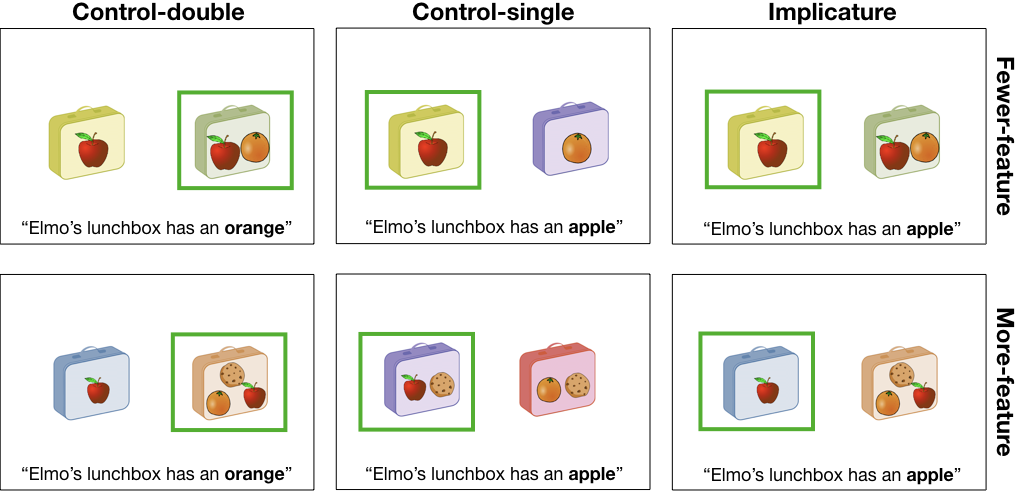
\includegraphics[width=5.98in]{figs/stimuli} \caption{Trial types. Green box indicates the target referent for each trial given the utterance at the bottom.}\label{fig:stimuli}
\end{figure}

On each trial, participants saw two images: a target and distractor,
which could either be an item with a single feature (e.g.~a lunchbox
with only an apple or only an orange), or an item with double features
(e.g., a lunchbox with an apple and an orange). In each trial, a
pre-recorded voice said a sentence (e.g., \enquote{Look at these
lunchboxes. Elmo's lunchbox has an apple.}). After participants chose
the object that was being referred to, a green box appeared around the
chosen object to show that the choice had been made. For each trial, we
recorded the participant's accuracy, or whether he or she selected the
correct target referent, and reaction time, or time spent between naming
of the referent (\enquote{\ldots{}an \emph{apple}}) and the
participant's referent selection.

There were three types of test trials (shown at the top of each panel in
Figure \ref{fig:stimuli}). In \emph{implicature} trials, the target item
had a single feature (e.g., an apple), and the distractor item had two
or three features (see below for the manipulation of number of features)
-- one that was in common with the target (e.g., an apple) and the other
feature(s) that was/were unique (e.g., an orange). The test sentence
named the feature that was common to the target and distractor. Thus, if
participants understood that \enquote{Elmo's lunchbox has an apple}
implicates \enquote{Elmo's lunchbox has an apple \emph{but not an
orange}} in the given context, it was predicted that they would choose
the target more often than the distractor; otherwise, if they did not
make implicatures, they would choose the two at equal rates (or even
choose the distractor more often depending on the degree of saliency
contrast -- see below).

There were two additional trial types, with semantically unambiguous
targets: \emph{Control-double} trials looked identical to implicature
trials, but the target and distractor were switched, such that the
double-feature item was the target and the single-feature item was the
distractor, and the test sentence named the unique feature on the
target. \emph{Control-single} trials presented two items that each had a
unique single feature, and either could be the target. Children saw 4
implicature, 4 control-double, and 8 control-single trials; adults saw 6
implicature, 6 control-double, and 12 control-single trials.

Each trial type was further divided by the number of features present on
the target and distractor (shown on the right side of Figure
\ref{fig:stimuli}): Within implicature trials, \emph{fewer-feature}
(2-vs-1) trials presented two features (an apple and an orange) on the
distractor and one feature (an apple) on the target, whereas
\emph{more-feature} (3-vs-1) trials presented three features (an apple,
an orange, and a cookie) on the distractor and one feature on the
target; Within control-double trials, \emph{fewer-feature} (2-vs-1)
trials presented two features (an apple and an orange) on the target and
one feature (an apple) on the distractor, whereas \emph{more-feature}
(3-vs-1) trials presented three features (an apple, an orange, and a
cookie) on the distractor and one feature on the target; Lastly, within
control-single trials, \emph{fewer-feature} (1-vs-1) trials presented
one feature each on the distractor and the target, whereas
\emph{more-feature} (2-vs-2) trials presented two features each on the
distractor and on the target. We hypothesized that older children would
choose the target more often in the more-feature implicature trials than
the fewer-feature implicature trials due to the strengthening of
implicatures -- \enquote{Elmo's lunchbox has an apple} is more likely to
mean \enquote{apple only} given an orange AND cookie on the alternative
referent, thus more things that could have been named but were not. On
the contrary, younger children were predicted to choose the target less
often in the more-feature trials than the fewer-feature trials due to
increased saliency of the distractor.

There were six sets of item and feature types, and the features were
named with nouns found on the MacArthur-Bates Communicative Development
Inventory word list (Fenson et al., 1994). Two orders of the test trials
were created, such that trial types and item types were counterbalanced
and trial order was pseudo-randomized across the two orders.

\subsection{Procedure}\label{procedure}

An experimenter introduced children to the task as a game on a tablet.
Then they completed two practice trials, where they were asked to select
an obvious, unambiguous referent (e.g., \enquote{cow} as opposed to
\enquote{rabbit}), followed by 16 test trials.

\subsection{Data analysis}\label{data-analysis}

We used R (Version 3.4.3; R Core Team, 2017) and the R-packages
\emph{bindrcpp} (Version 0.2; Müller, 2017a), \emph{brms} (Version
2.0.1; Bürkner, 2017), \emph{dplyr} (Version 0.7.4; Wickham, Francois,
Henry, \& Müller, 2017), \emph{forcats} (Version 0.2.0; Wickham, 2017a),
\emph{ggplot2} (Version 3.0.0; Wickham, 2009), \emph{ggthemes} (Version
3.4.0; Arnold, 2017), \emph{here} (Version 0.1; Müller, 2017b),
\emph{langcog} (Version 0.1.9001; Braginsky, Yurovsky, \& Frank, n.d.),
\emph{lme4} (Version 1.1.15; D. Bates, Mächler, Bolker, \& Walker,
2015), \emph{Matrix} (Version 1.2.12; D. Bates \& Maechler, 2017),
\emph{papaja} (Version 0.1.0.9655; Aust \& Barth, 2017), \emph{purrr}
(Version 0.2.4; Henry \& Wickham, 2017), \emph{Rcpp} (Eddelbuettel \&
Balamuta, 2017; Version 0.12.17; Eddelbuettel \& François, 2011),
\emph{readr} (Version 1.1.1; Wickham, Hester, \& Francois, 2017),
\emph{stringr} (Version 1.3.1; Wickham, 2017b), \emph{tibble} (Version
1.4.2; Müller \& Wickham, 2017), \emph{tidyr} (Version 0.7.2; Wickham \&
Henry, 2017), \emph{tidyverse} (Version 1.2.1; Wickham, 2017c), and
\emph{xtable} (Version 1.8.2; Dahl, 2016) for all our analyses.

\section{Results}\label{results}

We were interested in children's processing of implicatures in
comparison to unambiguous utterances, and developmental gains across
ages. We used two different measures: (1) accuracy and (2) reaction time
for choosing the correct referent. For each measure, we asked: (a) do
children show developmental gains in selection of the target referent?
And (b) does children's performance vary depending on salience contrast?
That is, when there are a relatively greater number of features on the
distractor, do children have more difficulty and are they slower in
choosing the correct referent?

As per our standard operating procedures, we removed trials in which the
log of reaction time was more than 3 standard deviations above or below
the mean (upper bound: 14.04 seconds; lower bound: 0.47 second;
percentage of data excluded: 1.67 \%). Throughout this section, we used
Bayesian linear mixed-effects models (\texttt{brms} package in R;
Bürkner, 2017) using crossed random effects of participant, item, and
sample (original vs.~replicationn) with the maximal random effects
structure supported by the design (Barr, Levy, Scheepers, \& Tily, 2013;
A. Gelman \& Hill, 2006). Age is plotted in year bins, but was analyzed
as a continuous variable, scaled and centered, in our statistical model.

\begin{figure}
\centering
\includegraphics{simpimp_paper_files/figure-latex/accuracy-1.pdf}
\caption{\label{fig:accuracy}Proportion of 2- to 5-year-old children
selecting the target in the original and replication samples (rows) in
different trial types (columns). Data are binned into 6-month age groups
for visualization purposes (all analyses are conducted on continuous
data). Lines are loess smoothing functions. Blue lines represent trials
in which there were fewer features present (2-vs-1 for control-double
and implicature, 1-vs-1 for control-single) and red lines represent
trials with more features (3-vs-1 for control-double and implicature,
2-vs-2 for control-single). Error bars are 95\% confidence intervals,
and are placed at the mean of the age bin and offset slightly to avoid
overplotting. Dashed line represents a conservative chance level at
50\%.}
\end{figure}

\subsection{Accuracy}\label{accuracy}

\begin{table}[tbp]
\begin{center}
\begin{threeparttable}
\caption{\label{tab:brmacc}Predictor mean estimates with standard deviation and 95\% credible interval information for a Bayesian linear mixed-effects model predicting accurate selection of target.}
\begin{tabular}{lllll}
\toprule
Predictor & \multicolumn{1}{c}{Mean} & \multicolumn{1}{c}{SD} & \multicolumn{1}{c}{95\% CI-Lower} & \multicolumn{1}{c}{95\% CI-Upper}\\
\midrule
Intercept & 4.60 & 3.86 & -4.94 & 11.71\\
Age & 2.30 & 3.80 & -5.84 & 10.06\\
Control-double & -0.07 & 3.53 & -7.86 & 7.71\\
Implicature & -3.33 & 4.41 & -13.11 & 4.46\\
More features & -0.68 & 3.70 & -9.83 & 5.81\\
Control-double * Age & -0.72 & 0.38 & -1.46 & 0.03\\
Implicature * Age & -1.00 & 0.38 & -1.77 & -0.29\\
More features * Age & -0.59 & 0.35 & -1.28 & 0.09\\
Control-double * More features & -0.06 & 0.56 & -1.16 & 1.02\\
Implicature * More features & 0.23 & 0.63 & -1.00 & 1.46\\
Control-double * Age * More features & 0.66 & 0.41 & -0.13 & 1.49\\
Implicature * Age * More features & 1.16 & 0.44 & 0.32 & 2.02\\
\bottomrule
\end{tabular}
\end{threeparttable}
\end{center}
\end{table}

The analysis of the accuracy rate (Figure \ref{fig:accuracy}) showed
that children across all ages were able to identify the target in
control trials, indicating that, as expected, they can readily compute
unambiguous meanings. In implicature trials, 4- and 5-year-olds'
performances were nearly at ceiling, replicating the previous results
(Horowitz et al., in press; Stiller et al., 2015). In our paradigm, even
3-year-olds chose the inferential target above chance\footnote{Because
  our task is a two-alternative forced choice, we define chance to be
  50\% across all trials. This baseline is a standard comparison that
  reflects the possibility that a child was completely inattentive to
  the task and chose completely at random. This baseline is more
  conservative than a salience-based baseline, which would likely
  suggest that the correct (inferentially-consistent) target would be
  chosen less than 50\% of the time (e.g., the \enquote{mumble}
  condition in Stiller et al., 2015).} (original sample: \(t\)(58) =
6.82, \(p\) \textless{} 0.001; replication sample: \(t\)(57) = 5.33,
\(p\) \textless{} 0.001). On the other hand, 2-year-olds' performance in
implicature trials did not differ from chance overall, but their
performance varied depending on the number of features present. In
3-vs-1 trials (i.e., with a relatively greater number of features on the
distractor), 2-year-olds did not choose the correct target referent, and
even tended to choose the distractor somewhat more often numerically
(original sample: \(t\)(23) = -1.42, \(p\) = 0.17; replication sample:
\(t\)(24) = -0.72, \(p\) = 0.48). However, In 2-vs-1 trials (with fewer
features on the distractor), 2-year-olds tended to choose the target
more often than the distractor. This difference was numerically present
in both samples and statistically significant in one (original sample:
\(t\)(26) = 0.46, \(p\) = 0.65; replication sample: \(t\)(24) = 2.57,
\(p\) = 0.02). By 4 years, this difference in accuracy rate between
2-vs-1 and 3-vs-1 trials was not present.

A Bayesian linear mixed-effects model predicting accuracy based on age,
trial type and number of features (salience contrast; more-feature
vs.~fewer-feature) showed a three-way positive interaction of age,
implicature trials, and number of features (Table \ref{tab:brmacc}).
Thus, unlike control trials, in which children's performances did not
differ by salience contrast, implicature trials showed lower accuracy in
3-vs-1 than 2-vs-1 trials in younger children, but not in older
children. This result supports our initial hypothesis that salience
contrast may lead to a greater struggle for younger children with the
implicature task due to a higher demand for inhibiting response to
distractor with greater salience.

\subsection{Reaction time}\label{reaction-time}

\begin{figure}
\centering
\includegraphics{simpimp_paper_files/figure-latex/rt-1.pdf}
\caption{\label{fig:rt}Reaction time to select the correct target referent.
Conventions are identical to Figure 2.}
\end{figure}

\begin{table}[tbp]
\begin{center}
\begin{threeparttable}
\caption{\label{tab:brmrt}Predictor mean estimates with standard deviation and 95\% credible interval information for a Bayesian linear mixed-effects model predicting log reaction time to select the target.}
\begin{tabular}{lllll}
\toprule
Predictor & \multicolumn{1}{c}{Mean} & \multicolumn{1}{c}{SD} & \multicolumn{1}{c}{95\% CI-Lower} & \multicolumn{1}{c}{95\% CI-Upper}\\
\midrule
Intercept & 7.80 & 2.24 & 3.19 & 12.79\\
Age & -0.22 & 2.83 & -6.43 & 5.97\\
Control-double & 0.02 & 3.16 & -6.98 & 6.05\\
Implicature & -0.05 & 3.65 & -8.44 & 6.01\\
More features & 0.25 & 2.67 & -4.92 & 6.56\\
Control-double * Age & -0.03 & 0.02 & -0.07 & 0.02\\
Implicature * Age & 0.09 & 0.03 & 0.04 & 0.14\\
More features * Age & 0.02 & 0.02 & -0.02 & 0.07\\
Control-double * More features & 0.09 & 0.04 & 0.02 & 0.17\\
Implicature * More features & -0.04 & 0.06 & -0.15 & 0.07\\
Control-double * Age * More features & 0.01 & 0.03 & -0.05 & 0.06\\
Implicature * Age * More features & -0.07 & 0.04 & -0.13 & 0.00\\
\bottomrule
\end{tabular}
\end{threeparttable}
\end{center}
\end{table}

With increasing age, children computed both implicatures and unambiguous
meanings and identified the target faster (Figure \ref{fig:rt}). A
Bayesian linear mixed-effects model predicting reaction time based on
age, trial type and number of features present showed a positive two-way
interaction between age and implicature trial (Table \ref{tab:brmrt}),
indicating that the speed of implicature computation did not improve
with age as much as the speed of processing unambiguous meanings.
Together with the accuracy finding, this result suggests that though
children become proficient at determining the \emph{correct} target
referents for ad-hoc implicatures by 5 years, implicature processing
develops relatively more slowly.

We also observed a positive two-way interaction between control-double
trials and number of features, indicating that children took longer to
identify the target in control-double trials with more features than in
control-single trials with more features. Interestingly, there was no
interaction between inference trials and number of features, or between
inference trial, age and number of features. Why would this be? We did
not have a pre-specified hypothesis regarding this pattern of data, but
we speculate that once a feature is named (e.g., Elmo's lunchbox has an
apple), it is relatively easier to find the feature in an inferential
target image than in the distractor image. The target feature is by
itself in the target referent, whereas it is grouped with with other
features in the distractor. Thus, the inference trials may allow easy
perceptual access to the target feature but also competition with the
overall perceptual salience of the distractor. These factors might
cancel one another out and lead to undifferentiated reaction times and
hence the lack of reaction time interactions. The potential advantage of
identifying a feature when it is by itself is only speculative, however,
and should be examined further in future work.

\section{Discussion}\label{discussion}

In our experiment, we confirmed 3- to 5-year-old children's successes on
ad-hoc implicature computation, and saw substantial developmental gains
in their accuracy and speed. 4- and 5-year-old children successfully
computed ad-hoc implicatures and identified the inferential targets,
consistent with previous findings. We found evidence of successful
implicature computation even in 3-year-olds. Between 2 and 5 years,
there was a clear improvement in processing skills with increasing age,
such that correct referent identification was more accurate and faster
across both control and implicature trials. Thus, these findings add to
the existing literature to attest to children's growing proficiency in
pragmatic processing.

We also investigated the salience hypothesis, namely that one cause of
young children's struggle with implicatures stems from their difficulty
to inhibit choosing the more salient distractor. In earlier work, there
was some numerical suggestion of 2-year-olds' preference for the more
salient but pragmatically incorrect distractor (Stiller et al., 2015).
We predicted that increasing the salience of this distractor would
result in decreased performance for younger children while increasing
performance for older children. The first part of this prediction was
clearly supported in our data, with younger children performing worse
when the distractor was more salient. Although we observed numerical
hints of a gain in accuracy for older children in one sample, we did not
see a consistent facilitation effect. We suspect this finding is due to
a ceiling effect: Referent selection via ad-hoc implicature is
relatively trivial for four-year-olds (Horowitz et al., in press).
However, we saw a possible age-related advantage of pragmatic
strengthening in the speed of computation: Whereas younger children
tended to be slower in trials with a greater number of features for both
unambiguous and inferential meanings, older children began to close the
gap and become faster to compute implicatures given increased distractor
saliency.

The salience account is not mutually exclusive with the alternatives
hypothesis described above (Barner et al., 2011). Indeed, both are
likely true and likely contribute to children's difficulty with
implicatures to different degrees in different tasks and at different
ages. For more complex alternative sets, the challenge may primarily be
identifying the appropriate alternatives, while for simpler
alternatives, difficulties may lie primarily in overcoming the pull of
the stronger one.

Although our salience account is most manifest in the kind of simple
referent selection tasks we used here, we believe it applies more
broadly to implicature computation beyond the scope of these tasks. Any
pragmatic implicature requires an asymmetry in the \enquote{strength} of
the alternatives. In ad-hoc referent-selection contexts, the stronger
(more salient) alternative is the item with more features. In scalar
implicatures, the implicature that you ate \emph{some but not all of the
cookies} is only possible because there is a stronger alternative
(\enquote{all}). It remains an open empirical question whether the
salience mismatch account might explain children's difficulty with these
other cases of implicatures as well.

One further application of our account is to word learning contexts,
where children's learning of a novel word is facilitated when the target
referent is more (not less) salient than its alternative. For example,
Frank and Goodman (2014) used an analogous pragmatic inference paradigm
in a word learning context: Participants heard a novel label (e.g.,
\enquote{a dinosaur with a \emph{dax}}) used to describe an object with
two features (a dinosaur with a hat and a bandanna) in the presence of
another dinosaur that had one but not the other of the features (a
dinosaur with a hat only). 3- and 4-year-olds performed quite well in
mapping the novel label to the unique feature (which would make the
labeling more informative). In this paradigm, the novel label was being
mapped to the more, rather than less, salient object. Similarly, in
classic \enquote{mutual exclusivity} paradigms (Markman \& Wachtel,
1988), by around 18 months, participants succeed in mapping a novel
label to a novel object (Halberda, 2003). While the mechanisms
underlying this empirical phenomenon are complex, it is well-established
that the salience of the novel target is an important factor in
children's success (see Markman, Wasow, \& Hansen, 2003 for discussion).
Overall, evidence for children's pragmatic word learning emerges earlier
than implicature computation: Children succeed in these tasks
substantially at earlier ages than even in our simplified implicature
paradigm. Our account suggests that one reason for this asymmetry is
because implicature tasks require selecting the \emph{less} salient
alternative while word learning tasks typically ask participants to
select a \emph{more} salient alternative.

Our findings help in the construction of a comprehensive developmental
account of processing of implicatures, and pragmatic inferences in
general. In the samples that have been studied in this literature, by 2
years of age, children begin to be aware that informativeness is
important to communication. Nevertheless, our findings suggest that the
salience contrasts inherent in many pragmatic situations may keep them
from successfully processing implicatures. Further, these same factors
are plausibly in play during pragmatic word learning tasks (Yurovsky \&
Frank, 2017). By 3 to 4 years, the ability to inhibit these salient
targets is more developed, and they start to compute ad-hoc implicatures
when relevant alternatives to the speaker's words are provided in
context. Scalar implicature performance develops more slowly, however,
as children's ability to access the relevant alternatives (and their
semantics) is only beginning to emerge (Barner et al., 2011; Horowitz et
al., in press; Skordos \& Papafragou, 2016); their performance during
these ages is highly variable and dependent on the nature of the context
and its pragmatic demands (Papafragou \& Tantalou, 2004).

One important challenge for this viewpoint is the nature of the ability
that children use to overcome the pull of the salient alternative. One
possible naive mapping for the ability would be to the broader construct
of executive function, which undergoes substantial developmental changes
during this period (Davidson et al., 2006; Diamond \& Taylor, 1996). But
executive function is a multi-faceted construct (Miyake et al., 2000),
and the particular components that would be expected to predict visual
(and perhaps conceptual) disengagement with a particular referent is
unclear. Our own studies attempting to probe individual difference
correlations between executive function and implicature ability in
development have not been successful (e.g., Horowitz et al., in press;
Nordmeyer, Yoon, \& Frank, 2016). Thus, a target for future work is to
better characterize the particular cognitive changes that relate to the
developmental effects we have observed here.

There are several further limitations of our work here. First, our
salience manipulation involved manipulation of the number of features
present on an item, which might have caused a potential confound between
salience and processing time. For example, children's greater looking to
the distractor might have been caused by a real desire to acquire more
information, rather than the mere perceptual salience of the
distractors. Second, as with nearly all work in the literature on
implicature processing, we address the performance of only relatively
high socioeconomic status children in a Western context. In our ongoing
work we address the generalizability of our task to other developmental
contexts (Fortier, Kellier, Fernández Flecha, \& Frank, in prep).

In sum, our work shows evidence that from at least 3 years, children are
able to compute ad-hoc implicatures, and that younger children's
failures with implicatures on an referent-choosing task are confounded
by the salience mismatch between possible referents. This pattern is
consistent with a broader generalization, namely that tasks that have
typically been used to look at children's implicature processing have a
variety of extraneous processing demands, which may explain why it has
been difficult to see children's underlying pragmatic abilities in such
paradigms. Thus, our work demonstrates the importance of using a range
of methods to measure children's pragmatic processing.

\newpage

\section{References}\label{references}

\setlength{\parindent}{-0.5in} \setlength{\leftskip}{0.5in}

\hypertarget{refs}{}
\hypertarget{ref-R-ggthemes}{}
Arnold, J. B. (2017). \emph{Ggthemes: Extra themes, scales and geoms for
'ggplot2'}. Retrieved from
\url{https://CRAN.R-project.org/package=ggthemes}

\hypertarget{ref-R-papaja}{}
Aust, F., \& Barth, M. (2017). \emph{papaja: Create APA manuscripts with
R Markdown}. Retrieved from \url{https://github.com/crsh/papaja}

\hypertarget{ref-barner2011}{}
Barner, D., Brooks, N., \& Bale, A. (2011). Accessing the unsaid: The
role of scalar alternatives in children's pragmatic inference.
\emph{Cognition}, \emph{118}(1), 84--93.
doi:\href{https://doi.org/10.1016/j.cognition.2010.10.010}{10.1016/j.cognition.2010.10.010}

\hypertarget{ref-barner2009}{}
Barner, D., Chow, K., \& Yang, S.-J. (2009). Finding one's meaning: A
test of the relation between quantifiers and integers in language
development. \emph{Cognitive Psychology}, \emph{58}(2), 195--219.
doi:\href{https://doi.org/10.1016/j.cogpsych.2008.07.001}{10.1016/j.cogpsych.2008.07.001}

\hypertarget{ref-barr2013random}{}
Barr, D. J., Levy, R., Scheepers, C., \& Tily, H. J. (2013). Random
effects structure for confirmatory hypothesis testing: Keep it maximal.
\emph{Journal of Memory and Language}, \emph{68}(3), 255--278.

\hypertarget{ref-R-Matrix}{}
Bates, D., \& Maechler, M. (2017). \emph{Matrix: Sparse and dense matrix
classes and methods}. Retrieved from
\url{https://CRAN.R-project.org/package=Matrix}

\hypertarget{ref-R-lme4}{}
Bates, D., Mächler, M., Bolker, B., \& Walker, S. (2015). Fitting linear
mixed-effects models using lme4. \emph{Journal of Statistical Software},
\emph{67}(1), 1--48.
doi:\href{https://doi.org/10.18637/jss.v067.i01}{10.18637/jss.v067.i01}

\hypertarget{ref-bott2012}{}
Bott, L., Bailey, T. M., \& Grodner, D. (2012). Distinguishing speed
from accuracy in scalar implicatures. \emph{Journal of Memory and
Language}, \emph{66}(1), 123--142.
doi:\href{https://doi.org/10.1016/j.jml.2011.09.005}{10.1016/j.jml.2011.09.005}

\hypertarget{ref-R-langcog}{}
Braginsky, M., Yurovsky, D., \& Frank, M. C. (n.d.). \emph{Langcog:
Language and cognition lab things}. Retrieved from
\url{http://github.com/langcog/langcog}

\hypertarget{ref-breheny2013}{}
Breheny, R., Ferguson, H. J., \& Katsos, N. (2013). Taking the epistemic
step: Toward a model of on-line access to conversational implicatures.
\emph{Cognition}, \emph{126}(3), 423--440.
doi:\href{https://doi.org/10.1016/j.cognition.2012.11.012}{10.1016/j.cognition.2012.11.012}

\hypertarget{ref-R-brms}{}
Bürkner, P.-C. (2017). brms: An R package for bayesian multilevel models
using Stan. \emph{Journal of Statistical Software}, \emph{80}(1), 1--28.
doi:\href{https://doi.org/10.18637/jss.v080.i01}{10.18637/jss.v080.i01}

\hypertarget{ref-chierchia2001}{}
Chierchia, G., Crain, S., Guasti, M. T., Gualmini, A., \& Meroni, L.
(2001). The acquisition of disjunction: Evidence for a grammatical view
of scalar implicatures. In \emph{Proceedings of BUCLD 25} (Vol. 157, p.
168).

\hypertarget{ref-R-xtable}{}
Dahl, D. B. (2016). \emph{Xtable: Export tables to latex or html}.
Retrieved from \url{https://CRAN.R-project.org/package=xtable}

\hypertarget{ref-davidson2006}{}
Davidson, M. C., Amso, D., Anderson, L. C., \& Diamond, A. (2006).
Development of cognitive control and executive functions from 4 to 13
years: Evidence from manipulations of memory, inhibition, and task
switching. \emph{Neuropsychologia}, \emph{44}(11), 2037--2078.
doi:\href{https://doi.org/10.1016/j.neuropsychologia.2006.02.006}{10.1016/j.neuropsychologia.2006.02.006}

\hypertarget{ref-diamond1996}{}
Diamond, A., \& Taylor, C. (1996). Development of an aspect of executive
control: Development of the abilities to remember what I said and to
``do as I say, not as I do''. \emph{Developmental Psychobiology},
\emph{29}, 315--334.
doi:\href{https://doi.org/10.1002/(SICI)1098-2302(199605)29:4/\%3C315::AID-DEV2/\%3E3.3.CO;2-C}{10.1002/(SICI)1098-2302(199605)29:4\textbackslash{}\%3C315::AID-DEV2\textbackslash{}\%3E3.3.CO;2-C}

\hypertarget{ref-R-Rcpp_b}{}
Eddelbuettel, D., \& Balamuta, J. J. (2017). Extending extitR with
extitC++: A Brief Introduction to extitRcpp. \emph{PeerJ Preprints},
\emph{5}, e3188v1.
doi:\href{https://doi.org/10.7287/peerj.preprints.3188v1}{10.7287/peerj.preprints.3188v1}

\hypertarget{ref-R-Rcpp_a}{}
Eddelbuettel, D., \& François, R. (2011). Rcpp: Seamless R and C++
integration. \emph{Journal of Statistical Software}, \emph{40}(8),
1--18.
doi:\href{https://doi.org/10.18637/jss.v040.i08}{10.18637/jss.v040.i08}

\hypertarget{ref-fenson1994}{}
Fenson, L., Dale, P. S., Reznick, J. S., Bates, E., Thal, D. J.,
Pethick, S. J., \ldots{} Stiles, J. (1994). Variability in early
communicative development. \emph{Monographs of the Society for Research
in Child Development}, i--185.
doi:\href{https://doi.org/10.2307/1166093}{10.2307/1166093}

\hypertarget{ref-fortierunderrev}{}
Fortier, M., Kellier, D., Fernández Flecha, M., \& Frank, M. C. (in
prep). Ad-hoc pragmatic implicatures among shipibo-konibo children in
the peruvian amazon.
doi:\href{https://doi.org/10.17605/OSF.IO/X7AD9}{10.17605/OSF.IO/X7AD9}

\hypertarget{ref-frank2012}{}
Frank, M. C., \& Goodman, N. D. (2012). Predicting pragmatic reasoning
in language games. \emph{Science}, \emph{336}(6084), 998--998.
doi:\href{https://doi.org/10.1016/j.cogpsych.2014.08.002}{10.1016/j.cogpsych.2014.08.002}

\hypertarget{ref-frank2014}{}
Frank, M. C., \& Goodman, N. D. (2014). Inferring word meanings by
assuming that speakers are informative. \emph{Cognitive Psychology},
\emph{75}, 80--96.
doi:\href{https://doi.org/10.1016/j.cogpsych.2014.08.002}{10.1016/j.cogpsych.2014.08.002}

\hypertarget{ref-frank2016}{}
Frank, M. C., Sugarman, E., Horowitz, A. C., Lewis, M. L., \& Yurovsky,
D. (2016). Using tablets to collect data from young children.
\emph{Journal of Cognition and Development}, \emph{17}, 1--17.
doi:\href{https://doi.org/10.1080/15248372.2015.1061528}{10.1080/15248372.2015.1061528}

\hypertarget{ref-gelman2006data}{}
Gelman, A., \& Hill, J. (2006). \emph{Data analysis using regression and
multilevel/hierarchical models}. Cambridge university press.

\hypertarget{ref-goodman2016}{}
Goodman, N. D., \& Frank, M. C. (2016). Pragmatic language
interpretation as probabilistic inference. \emph{Trends in Cognitive
Sciences}, \emph{20}(11), 818--829.

\hypertarget{ref-grice1975logic}{}
Grice, H. P. (1975). Logic and conversation. \emph{Syntax and
Semantics}, \emph{3}, 41--58.

\hypertarget{ref-grodner2010}{}
Grodner, D. J., Klein, N. M., Carbary, K. M., \& Tanenhaus, M. K.
(2010). ?Some,? And possibly all, scalar inferences are not delayed:
Evidence for immediate pragmatic enrichment. \emph{Cognition},
\emph{116}(1), 42--55.

\hypertarget{ref-halberda2003development}{}
Halberda, J. (2003). The development of a word-learning strategy.
\emph{Cognition}, \emph{87}(1), B23--B34.

\hypertarget{ref-R-purrr}{}
Henry, L., \& Wickham, H. (2017). \emph{Purrr: Functional programming
tools}. Retrieved from \url{https://CRAN.R-project.org/package=purrr}

\hypertarget{ref-horowitzSchneider}{}
Horowitz, A. C., Schneider, R. M., \& Frank, M. C. (in press). The
trouble with quantifiers: Explaining children's deficits in scalar
implicature. \emph{Child Development}.

\hypertarget{ref-huang2009b}{}
Huang, Y. T., \& Snedeker, J. (2009). Semantic meaning and pragmatic
interpretation in 5-year-olds: Evidence from real-time spoken language
comprehension. \emph{Developmental Psychology}, \emph{45}(6), 1723.
doi:\href{https://doi.org/10.1037/a0016704}{10.1037/a0016704}

\hypertarget{ref-huang2018}{}
Huang, Y. T., \& Snedeker, J. (2018). Some inferences still take time:
Prosody, predictability, and the speed of scalar implicatures.
\emph{Cognitive Psychology}, \emph{102}, 105--126.

\hypertarget{ref-hurewitz2006}{}
Hurewitz, F., Papafragou, A., Gleitman, L., \& Gelman, R. (2006).
Asymmetries in the acquisition of numbers and quantifiers.
\emph{Language Learning and Development}, \emph{2}(2), 77--96.
doi:\href{https://doi.org/10.1207/s15473341lld0202_1}{10.1207/s15473341lld0202\_1}

\hypertarget{ref-katsos2011}{}
Katsos, N., \& Bishop, D. V. (2011). Pragmatic tolerance: Implications
for the acquisition of informativeness and implicature.
\emph{Cognition}, \emph{120}(1), 67--81.
doi:\href{https://doi.org/10.1016/j.cognition.2011.02.015}{10.1016/j.cognition.2011.02.015}

\hypertarget{ref-markman1988children}{}
Markman, E. M., \& Wachtel, G. F. (1988). Children's use of mutual
exclusivity to constrain the meanings of words. \emph{Cognitive
Psychology}, \emph{20}(2), 121--157.

\hypertarget{ref-markman2003use}{}
Markman, E. M., Wasow, J. L., \& Hansen, M. B. (2003). Use of the mutual
exclusivity assumption by young word learners. \emph{Cognitive
Psychology}, \emph{47}(3), 241--275.

\hypertarget{ref-matthews2012}{}
Matthews, D., Butcher, J., Lieven, E., \& Tomasello, M. (2012). Two-and
four-year-olds learn to adapt referring expressions to context: Effects
of distracters and feedback on referential communication. \emph{Topics
in Cognitive Science}, \emph{4}(2), 184--210.
doi:\href{https://doi.org/10.1111/j.1756-8765.2012.01181.x}{10.1111/j.1756-8765.2012.01181.x}

\hypertarget{ref-miyake2000unity}{}
Miyake, A., Friedman, N. P., Emerson, M. J., Witzki, A. H., Howerter,
A., \& Wager, T. D. (2000). The unity and diversity of executive
functions and their contributions to complex ``frontal lobe'' tasks: A
latent variable analysis. \emph{Cognitive Psychology}, \emph{41}(1),
49--100.

\hypertarget{ref-R-bindrcpp}{}
Müller, K. (2017a). \emph{Bindrcpp: An 'rcpp' interface to active
bindings}. Retrieved from
\url{https://CRAN.R-project.org/package=bindrcpp}

\hypertarget{ref-R-here}{}
Müller, K. (2017b). \emph{Here: A simpler way to find your files}.
Retrieved from \url{https://CRAN.R-project.org/package=here}

\hypertarget{ref-R-tibble}{}
Müller, K., \& Wickham, H. (2017). \emph{Tibble: Simple data frames}.
Retrieved from \url{https://CRAN.R-project.org/package=tibble}

\hypertarget{ref-nordmeyer2016}{}
Nordmeyer, A. E., Yoon, E. J., \& Frank, M. C. (2016). Distinguishing
processing difficulties in inhibition, implicature, and negation. In
\emph{Proceedings of the 38th annual meeting of the cognitive science
society}.

\hypertarget{ref-noveck2001}{}
Noveck, I. A. (2001). When children are more logical than adults:
Experimental investigations of scalar implicature. \emph{Cognition},
\emph{78}(2), 165--188.
doi:\href{https://doi.org/10.1016/S0010-0277(00)00114-1}{10.1016/S0010-0277(00)00114-1}

\hypertarget{ref-oneill2001}{}
O'Neill, D. K., \& Topolovec, J. C. (2001). Two-year-old children's
sensitivity to the referential (in) efficacy of their own pointing
gestures. \emph{Journal of Child Language}, \emph{28}(1), 1--28.
doi:\href{https://doi.org/10.1017/S0305000900004566}{10.1017/S0305000900004566}

\hypertarget{ref-papafragou2003}{}
Papafragou, A., \& Musolino, J. (2003). Scalar implicatures: Experiments
at the semantics--pragmatics interface. \emph{Cognition}, \emph{86}(3),
253--282.
doi:\href{https://doi.org/10.1016/S0010-0277(02)00179-8}{10.1016/S0010-0277(02)00179-8}

\hypertarget{ref-papafragou2004}{}
Papafragou, A., \& Tantalou, N. (2004). Children's computation of
implicatures. \emph{Language Acquisition}, \emph{12}(1), 71--82.
doi:\href{https://doi.org/10.1207/s15327817la1201_3}{10.1207/s15327817la1201\_3}

\hypertarget{ref-R-base}{}
R Core Team. (2017). \emph{R: A language and environment for statistical
computing}. Vienna, Austria: R Foundation for Statistical Computing.
Retrieved from \url{https://www.R-project.org/}

\hypertarget{ref-simmons2011false}{}
Simmons, J. P., Nelson, L. D., \& Simonsohn, U. (2011). False-positive
psychology: Undisclosed flexibility in data collection and analysis
allows presenting anything as significant. \emph{Psychological Science},
\emph{22}(11), 1359--1366.

\hypertarget{ref-skordos2016}{}
Skordos, D., \& Papafragou, A. (2016). Children's derivation of scalar
implicatures: Alternatives and relevance. \emph{Cognition}, \emph{153},
6--18.
doi:\href{https://doi.org/10.1016/j.cognition.2016.04.006}{10.1016/j.cognition.2016.04.006}

\hypertarget{ref-sperber1986}{}
Sperber, D., \& Wilson, D. (1995). \emph{Relevance: Communication and
cognition}. Oxford: Blackwell.

\hypertarget{ref-stiller2015}{}
Stiller, A., Goodman, N. D., \& Frank, M. C. (2015). Ad-hoc implicature
in preschool children. \emph{Language Learning and Development}.
doi:\href{https://doi.org/10.1080/15475441.2014.927328}{10.1080/15475441.2014.927328}

\hypertarget{ref-R-ggplot2}{}
Wickham, H. (2009). \emph{Ggplot2: Elegant graphics for data analysis}.
Springer-Verlag New York. Retrieved from \url{http://ggplot2.org}

\hypertarget{ref-R-forcats}{}
Wickham, H. (2017a). \emph{Forcats: Tools for working with categorical
variables (factors)}. Retrieved from
\url{https://CRAN.R-project.org/package=forcats}

\hypertarget{ref-R-stringr}{}
Wickham, H. (2017b). \emph{Stringr: Simple, consistent wrappers for
common string operations}. Retrieved from
\url{https://CRAN.R-project.org/package=stringr}

\hypertarget{ref-R-tidyverse}{}
Wickham, H. (2017c). \emph{Tidyverse: Easily install and load the
'tidyverse'}. Retrieved from
\url{https://CRAN.R-project.org/package=tidyverse}

\hypertarget{ref-R-tidyr}{}
Wickham, H., \& Henry, L. (2017). \emph{Tidyr: Easily tidy data with
'spread()' and 'gather()' functions}. Retrieved from
\url{https://CRAN.R-project.org/package=tidyr}

\hypertarget{ref-R-dplyr}{}
Wickham, H., Francois, R., Henry, L., \& Müller, K. (2017). \emph{Dplyr:
A grammar of data manipulation}. Retrieved from
\url{https://CRAN.R-project.org/package=dplyr}

\hypertarget{ref-R-readr}{}
Wickham, H., Hester, J., \& Francois, R. (2017). \emph{Readr: Read
rectangular text data}. Retrieved from
\url{https://CRAN.R-project.org/package=readr}

\hypertarget{ref-yurovsky2017}{}
Yurovsky, D., \& Frank, M. C. (2017). Beyond naive cue combination:
Salience and social cues in early word learning. \emph{Developmental
Science}.
doi:\href{https://doi.org/10.1111/desc.12349}{10.1111/desc.12349}






\end{document}
